\documentclass{article}
\usepackage{graphicx}
\usepackage{hyperref}
\usepackage{pgfplots}
\usepackage{amsmath}
\graphicspath{{images/}}
\usepackage{amsthm}
\theoremstyle{definition}
\newtheorem{example}{Example}[section]
\usepackage{fancybox}
\usepackage[]{algorithm2e, algorithmic}
\makeatletter
\renewcommand{\@algocf@capt@plain}{above}% formerly {bottom}
\makeatother

\begin{document}

\title{Parallelizing Convex Learning Algorithms}
\author{Michael Curtis 260475694\\
Voula Theophanous 260480568}
\maketitle

\begin{abstract}

This report outlines methodologies for parallelizing convex cost function machine learning algorithms. We present a Master-Worker implementation and a Gradient-Gossip based implementation. Both of these methods aim to minimize the amount of communications between processes and maximize the amount of parallel execution. We will also describe what a convex function is, how convexity relates to learning algorithms, and why convex learning algorithms can be parallelized.

\end{abstract}

\section{Introduction}
The following example illustrates why executing machine learning algorithms faster could be important. Imagine you are a computer scientist for the World Health Organization. There has been an outbreak of a mosquito born virus that has been growing in western African countries. It has been found that spraying airborne pesticides to control misquito population is effective in controlling the spread of the virus. Your organization has 140 teams delegated to spraying the pesticides across the effected countries. You have over 3000 mosquito hotspots near population centers where mosquitos' blood have been testing at high rates for the virus. You are given the location of mosquito blood testing, associated rate of virus occurrence in mosquito and population centers, and previous pesticide sprays with associated location. You have decided to build a linear regression model aiming to minimize the total number of mosquito positive virus tests. Since there are hundreds or thousands of features in our training data the model takes days to build when running in serial. If we have a method to parallelize this learning algorithm we could send the 140 teams to an optimally chosen 140 of the 3000 locations in the magnitude of hours.

\subsection{Definition: Convex Functions}
The simple and informal definition of a convex function is to visualize a parabola, where we can easily see that there is only one global minimum. That is there is only one set of parameters to the derivative of the function that will return 0. Lets try to visualize this in general. Pick two sets of parameters to the function that given us two different points on the functions. With the two points draw a line connecting, or in the higher dimensional case, visualize a surface where both the points are contained. If for any two points of any parameters has an obstruction disallowing a line of sight from one point to another, the function is not convex as there will be multiple parameter values such that the derivative of the function evaluates to 0. This is mathematically defined in Stanford Professor Stephen Boyd's textbook\footnote{\url{https://web.stanford.edu/~boyd/cvxbook/bv_cvxbook.pdf}} \\
\\
A function $f:R^n \rightarrow R$ is \textit{convex} if $domain f$ is a convex set and if for all $x,y \in domain f$, and $\theta$ with $0 \leq \theta \leq 1$, we have
\begin{equation}
    \label{simple_equation}
    f(\theta x + (1 - \theta)y) \leq \theta f(x) + (1 - \theta)f(y)
\end{equation}
\begin{figure}[ht]
    \centering
    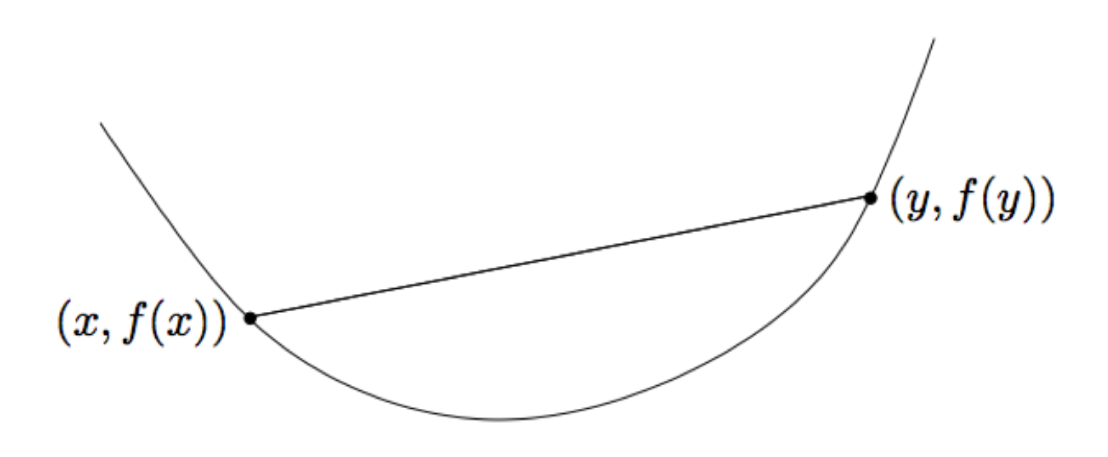
\includegraphics[width=3.0in]{convexboyd}
    \caption{A "chord" Between Two Points In a Convex Function}
    \label{convexboyd}
\end{figure}

\subsection{Convexity and Machine Learning}
The objective of learning algorithms is to build a model using a set of training data $X$ and target data $y$. The model can then take new $X$ data and output a prediction of $y$ data. In many cases describing the correlation between $X$ and $y$ is done by finding a weighting matrix $w$. As seen in figure 2\footnote{\url{http://cs.mcgill.ca/~jpineau/comp598/Lectures/02LinearRegression-publish.pdf}}, 
$
    w =
    \begin{bmatrix}
        w_{1}\\
        w_{2}\\
    \end{bmatrix}
    = 
    \begin{bmatrix}
        1.60\\
        1.05\\
    \end{bmatrix}
$. These algorithms search for the optimal weight matrix by minimizing the error between a generated model and the $X$, $y$ datapoints. Machine learning algorithms such as linear regression, support vector machines, LASSO linear regression, ridge regression, logistic regression, and metric learning all use \textbf{convex} cost functions to evaluate error.\\

\begin{figure}[!ht]
    \centering
    \begin{tikzpicture}
        \begin{axis} [
            ylabel = $y$, 
            xlabel = $x$,
            xmin = -1,
            xmax =  2,
            ymin = -1,
            ymax = 4
            ]
            \addplot+[only marks, mark=square]
            coordinates {
                (0.86, 2.49)
                (0.09, 0.83)
                (-0.85, -0.25)
                (0.87, 3.10)
                (0.44, 0.87)
                (-0.43, 0.02)
                (-1.10, -0.12)
                (0.40, 1.81)
                (-0.96, -0.83)
                (0.17, 0.43)
            };
            \addplot[color=red]{1.60*x + 1.05} node[above,pos=1] {$y = 1.60x + 1.05$};
        \end{axis}
    \end{tikzpicture}
    \caption[]{$w$ Describes The Line That Minimizes Error: $y = 1.60x + 1.05$}
    \label{wsolved}
\end{figure}

\begin{example}
    Linear regression builds a predictive model $Y = Xw$ by minimizing the least-squares, error evaluation function $error(w) = (Y - Xw)^T(Y - Xw)$. We minimize $error(w)$ by setting its derivative to zero and traversing potential $w_0, w_1, ... w_n$ values until we are within an acceptable range of zero. Where we find a $w$ such that $\frac{\partial error(w)}{\partial w} = -2X^T(Y - Xw) = 0$. This algorithm's output is illustrated in figure 2. Later in this report we will use linear regression to test our parallelization.
\end{example}

The key point of convexity as it relates to optimization of machine learning algorithms is that if a the error evaluation function is convex we can use a gradient descent algorithm to traverse the potential $w_0, w_1, ... w_n$ values. Even more crucial is the fact that gradient descent algorithms are parallelizible.

\begin{algorithm}[!ht]
    \SetAlgoLined
    \caption{Centralized Gradient Descent}
    given a starting point $w \in domain f$\;
    \Repeat{stopping criterion is satisfied}{
    1. $\Delta w := \nabla f(w)$\;
    2. Line Search. Choose step size $t$ via exact or backtracking line search.\;
    3. Update. $w := w + t\nabla f(w)$}
\end{algorithm}{

We can visualize Algorithm 1's execution via the convex definition given in Figure 1 where the our gradient descent is traversing weight paramater values $w_0, w_1, ... w_n$. The algorithm stops once it has found the global minimum.

\section{Master-Worker Parallelization}
\subsection{Implementation}
Each evaluation of $\Delta w := \nabla f(w)$ in step 1 of Algorithm 1 can be computationally heavy with a large $X$. Our algorithm separates $X$ into $X_0, X_1, ... ,X_n$ and associates $\nabla f(w)$'s with $n$ processes and thus, speeds up the time it takes for step 1 to execute on each iteration. Master-Worker delegates a single process to steps 2 and 3 of Algorithm 1, where each iteration's $w$ vector is assigned, as well as the comparison epsilon check to see if the algorithm has satisfied the stopping criterion. This master process sends the newly found $w$ to the $n$ worker processes delegated to evaluating their local $\Delta w := \nabla f_i(w)$ then each worker sends that value back to the master for reduction via the summation $\nabla f(w) = \nabla f_0(w) + \nabla f_1(w) + ... + \nabla f_n(w)$. Note that $\nabla f_i(w) = -2X_i^T(Y - X_iw)$ for $0 \leq i \leq n$ for our linear regression test example.

\subsection{Results}
In the smaller bike sharing  dataset we can see the parallel execution time decrease with the number of processes less than four but, become slower relative to the single process time as the number of processes increases past four. This is due to the larger percentage of communication vs computation given a smaller dataset. However, as the datasets grow in size, as we see in the second two twitter datasets, a speedup above one is always found regardless of the number of processes. This shows the master-worker implementation is effective in finding a significant speedup in parallelizing machine learning algorithms working with large datasets.
\clearpage
\subsubsection{Bike Sharing Dataset}
We used the Kaggle bike sharing competition database for our first test of the master-worker implementation. The $X$ data included 14000 datapoints with 12 features. 

\begin{figure}[!ht]
    \centering
    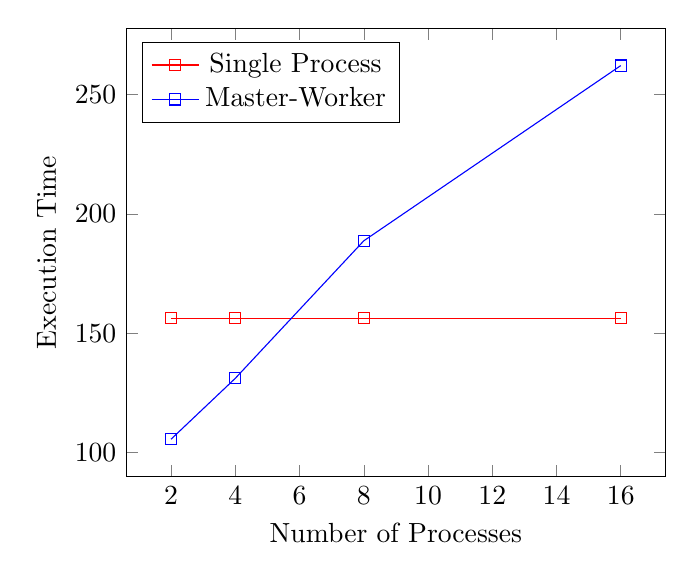
\begin{tikzpicture}
        \begin{axis} [
            legend pos=north west,
            ylabel = Execution Time, 
            xlabel = Number of Processes,
            ]
            \addplot+[color=red, mark=square]
            coordinates {
                (2, 156.317349)
                (4, 156.317349)
                (8, 156.317349)
                (16, 156.317349)
            };
            \addlegendentry{Single Process}
            \addplot+[color=blue, mark=square]
            coordinates {
                (2, 105.681159)
                (4, 131.170156)
                (8, 188.7401731)
                (16, 262.101258)
            };
            \addlegendentry{Master-Worker}
        \end{axis}
    \end{tikzpicture}
    \caption[]{Master-Worker Bike Sharing Data Execution Time}
    \label{bikesharing}
\end{figure}

\begin{figure}[!ht]
    \centering
    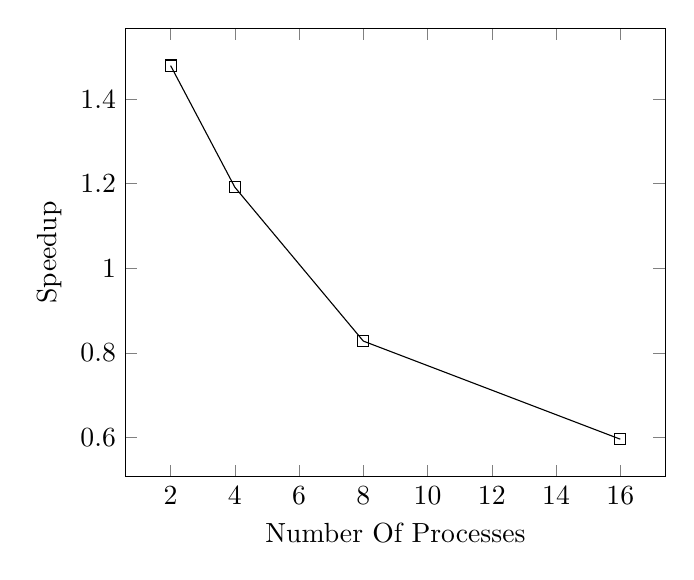
\begin{tikzpicture}
        \begin{axis} [
            ylabel = Speedup, 
            xlabel = Number Of Processes,
            ]
            \addplot+[color=black, mark=square]
            coordinates {
                (2, 1.47914113)
                (4, 1.191714287)
                (8, 0.828214505)
                (16, 0.596400605)
            };
        \end{axis}
    \end{tikzpicture}
    \caption[]{Master-Worker Bike Sharing Data Speedup}
    \label{bikesharing2}
\end{figure}


\subsubsection{Twitter Database 50k Datapoints}
The second test set we used was the a twitter feature set we scaled down to 50000 datapoints with 10 features. 

\begin{figure}[!ht]
    \centering
    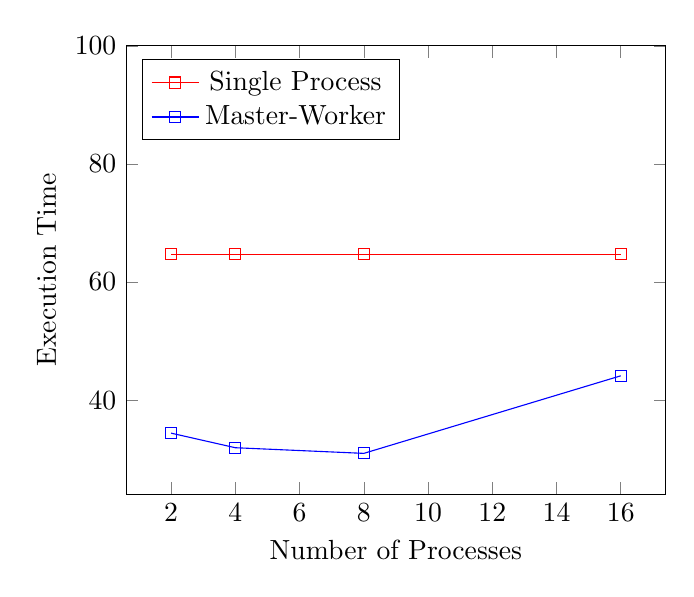
\begin{tikzpicture}
        \begin{axis} [
            legend pos=north west,
            ylabel = Execution Time, 
            xlabel = Number of Processes,
            ymax = 100,
            ]
            \addplot+[color=red, mark=square]
            coordinates {
                (2, 64.67645597)
                (4, 64.67645597)
                (8, 64.67645597)
                (16, 64.67645597)
            };
            \addlegendentry{Single Process}
            \addplot+[color=blue, mark=square]
            coordinates {
                (2, 34.40762401)
                (4, 31.93840504)
                (8, 30.98179698)
                (16, 44.11726999)
            };
            \addlegendentry{Master-Worker}
        \end{axis}
    \end{tikzpicture}
    \caption[]{Master-Worker 50k Twitter Data Execution Time}
    \label{50k}
\end{figure}

\begin{figure}[!ht]
    \centering
    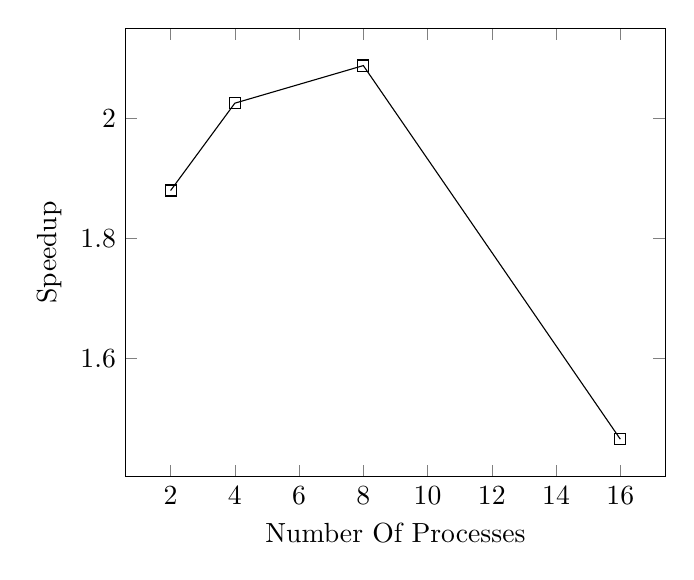
\begin{tikzpicture}
        \begin{axis} [
            ylabel = Speedup, 
            xlabel = Number Of Processes,
            ]
            \addplot+[color=black, mark=square]
            coordinates {
                (2, 1.879712937)
                (4, 2.025037127)
                (8, 2.087563094)
                (16, 1.466012199)
            };
        \end{axis}
    \end{tikzpicture}
    \caption[]{Master-Worker 50k Twitter Data Speedup}
    \label{50k2}
\end{figure}

\subsubsection{Twitter Database 100k Datapoints}
The third test set we used was the a twitter feature set we scaled down to 100000 datapoints with 10 features. 

\begin{figure}[!ht]
    \centering
    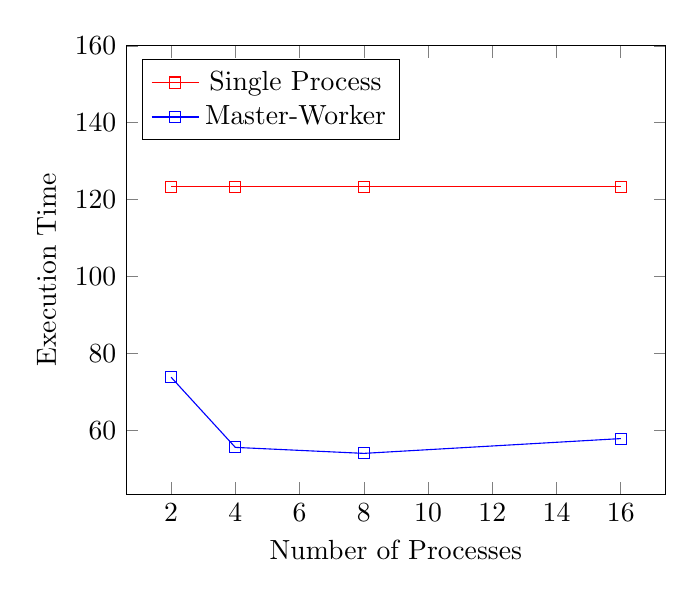
\begin{tikzpicture}
        \begin{axis} [
            legend pos=north west,
            ylabel = Execution Time, 
            xlabel = Number of Processes,
            ymax = 160,
            ]
            \addplot+[color=red, mark=square]
            coordinates {
                (2, 123.30112)
                (4, 123.30112)
                (8, 123.30112)
                (16, 123.30112)
            };
            \addlegendentry{Single Process}
            \addplot+[color=blue, mark=square]
            coordinates {
                (2, 73.79524112)
                (4, 55.53795195)
                (8, 53.9791162)
                (16, 57.82486796)
            };
            \addlegendentry{Master-Worker}
        \end{axis}
    \end{tikzpicture}
    \caption[]{Master-Worker 100k Twitter Data Execution Time}
    \label{100k}
\end{figure}

\begin{figure}[!ht]
    \centering
    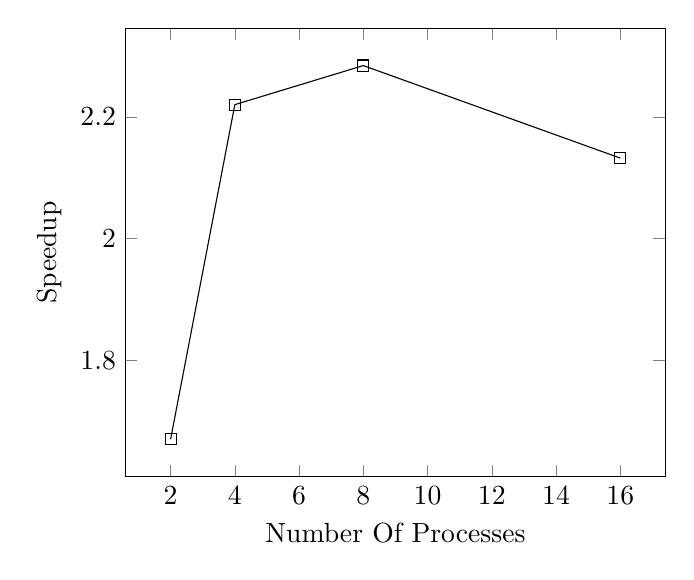
\begin{tikzpicture}
        \begin{axis} [
            ylabel = Speedup, 
            xlabel = Number Of Processes,
            ]
            \addplot+[color=black, mark=square]
            coordinates {
                (2, 1.670854627)
                (4, 2.22012364)
                (8, 2.284237474)
                (16, 2.132319958)
            };
        \end{axis}
    \end{tikzpicture}
    \caption[]{Master-Worker 100k Twitter Data Speedup}
    \label{100k2}
\end{figure}
\section{Synchronous Gossip Parallelization}
\subsection{Implementation}
Synchronous gossip is simliar to the master-worker implementation in that the machine learning cost functions are required to be convex for parallelization. Synchronous gossip is fundamentally different because it leaves the responsibility of finding a weight matrix $w_i$ to each process. In this section we will detail why all processes in the defined network would converge to the same solution for the weight matrix $w$. Algorithm 2 describes a process in which nodes compute gradients relative to their local gradient functions as defined by their $X_i$ data.

\begin{algorithm}[!ht]
    \SetAlgoLined
    \caption{Synchronous Gossip Gradient Descent}
    Neighbours at process $i$ are $N_i = \{j : (i,j)\in Edges\}\cup \{i\}$\;
    Weighting matrix at process $i$ is $x_0^i = [0, 0, ... 0]$\;
    \Repeat{stopping criterion is satisfied}{
    1. Compute $\nabla f_i(x^i_k)$\;
    2. Send $\nabla f_i(x^i_k)$ to neighbors\;
    3. Receive $\nabla f_i(x^j_k)$ from neighbors\;
    4. Update $x^i_{k+1} = x^i_k - \alpha_k \sum_{j\in N_i} w_{ij}\nabla f_j(x^j_k)$}
\end{algorithm}{

\subsubsection{Convergence Requirements}
Graph requirements for $G = (V, E)$:
\begin{enumerate}
    \item $G$ does not change
    \item $G$ is connected
    \item $G$ is undirected
    \item $w_{ij} = 0$ if $(i,j) \not\in E$ and $i \neq j$
    \item $\sum_{j\in N_i} w_{ij} = 1$ 
    \item $\sum_{i=1}^{n} w_{ij} = 1$
\end{enumerate}

\subsubsection{Communication Efficiency Requirements}
There are two major contributing factors in our implementation that directly relate to an increased speedup of execution. The first of which is to decide whether an edge exists between two processes by a probability that is a function of the number of processes. Overwhelming odds suggest that the graph created by this process, \textit{Erdos-Renyi Model} equation (\ref{erdos}), leads to a graph in which most nodes are connected by a edge distance of two. Having an average connection distance of two edges between two nodes allows for the most efficient communication of send and receives between processes.

\begin{equation}
    \label{erdos}
    Pr((i,j) \in E) = \sqrt{\frac{2log(n)}{n}}
\end{equation}

\begin{figure}[ht]
    \centering
    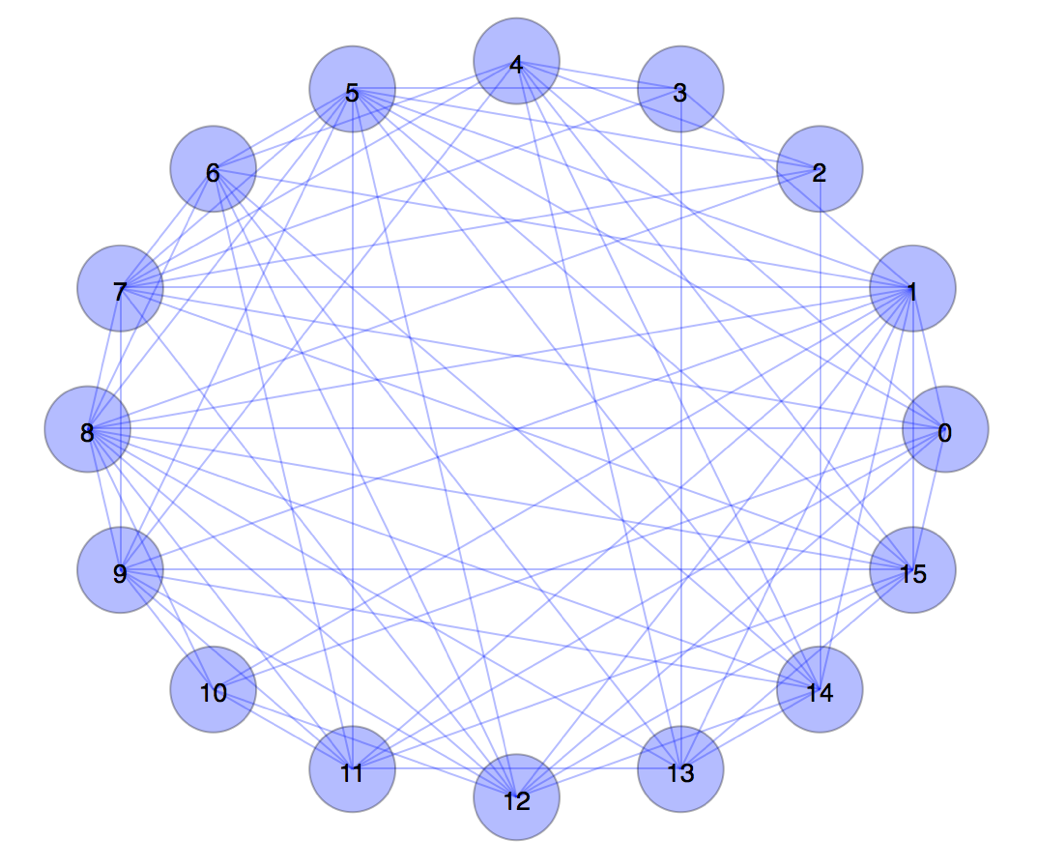
\includegraphics[width=3.0in]{graph}
    \caption{Graph Generated Via Erdos-Renyi Model}
    \label{graph}
\end{figure}

The second factor in allowing efficient communication in our synchronous gossip implementation is to assign edge weights in a way that leads to fast convergence. \textit{Metropolis-Hastings}, equation (\ref{mhweights}), assign weights via edge degrees. In other words processes that have more influence over multiple nodes' weight matrix give those processes more weighting to allow for faster communication of changes in the weights due to their local data.

\begin{equation}
    \label{mhweights}
    \begin{split}
        & \text{ For } i\neq j \text{ set } w_ij =\begin{cases}
        \frac{1}{max(deg(i),deg(j))}, & \text{if $(i,j) \in E$}.\\
        0, & \text{otherwise}.\\
        %\text{ For } i\eq j \text{ set } w_ij = 1 - \sum_{j=1}^{n} w_{ij}
      \end{cases} \\
      & \text{ For } i = j \text{ set } w_ij = 1 - \sum_{j=1}^{n} w_{ij}
  \end{split}
\end{equation}
\subsection{Results}
In our implementation we used another simple kaggle dataset that has only two features with a closed form linear regression solution of $w_0 = 938.238$ and $w_1 = 152.92$. Our synchronous gossip implementation used five processes as seen in the figure below to find a solution. 

\begin{figure}[ht]
    \centering
    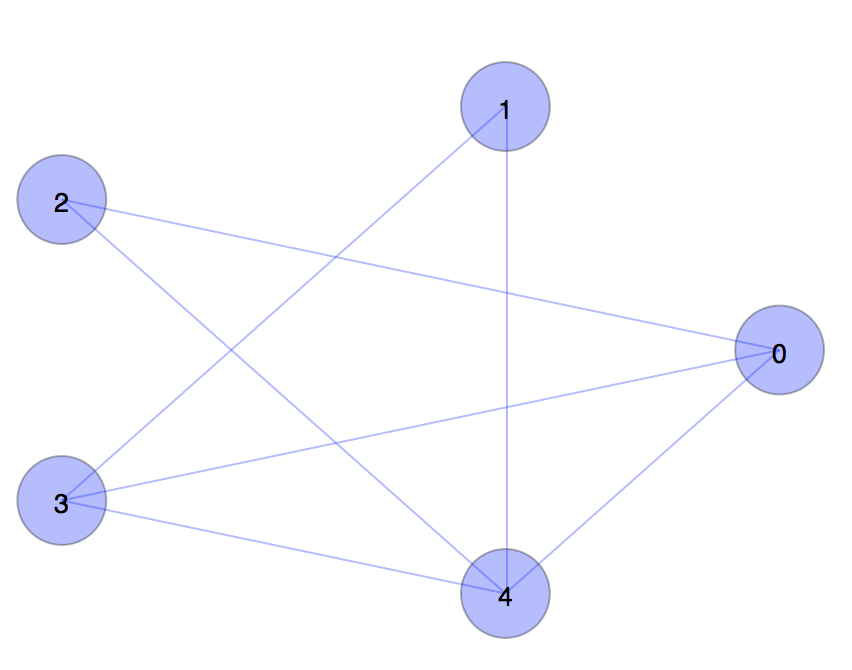
\includegraphics[width=3.0in]{five}
    \caption{Five Process Graph Generated For Synchronous Gossip Testing}
    \label{five}
\end{figure}

While each process converged to within a few decimal places of our closed form $w_0$ and $w_1$ we were unable to stop the algorithm in an efficient way to test for speedup. This is because the only trivial way to constantly test for stopping criterion is by adding a message for each process broadcasting that that specific process is completed. This would add a large overhead in terms of communication costs. We could have just killed the execution when one of the processes finished but this would not give us an accurate time measurement of the execution as only one of the processes would be done while others still need time to reach the stopping criterion.
\section{Conclusion}
The key introductory knowledge is that some machine learning algorithm have convex cost functions, where convex cost functions allow for gradient descent and gradient descent is parallelizable. With our master-worker implementation we were able to show significant speedups while our synchronous gossip implementation we showed that we can have multiple processes independently converge to a weighting matrix solution. Further research is required to determine the most efficient means of stopping the synchronous gossip implementation.

\end{document}
